\chapter{Alternatywne podejście do pisania aplikacji na platformę Adroid}
\label{propozycja_rozwiazania}

\section{Tworzenie aplikacji od podstaw}
\label{nowa_aplikacja}
\subsection{Nowe podejście do architektury systemu}
\label{clean_architecture}
Okazuje się, że największą przeszkodą w~testowaniu aplikacji androidowych jest Android sam w~sobie. Im większy \textit{coupling} między warstwami, tym trudniej jest pisać testy jednostkowe. Rozważmy więc przekształcenie modelu aplikacji Android opisanego w~rozdziale \ref{standardowe_podejscie} przedstawione na~rysunku \ref{fig:opis_rozwiazania}.

\begin{figure}[!htb]
    \centering
    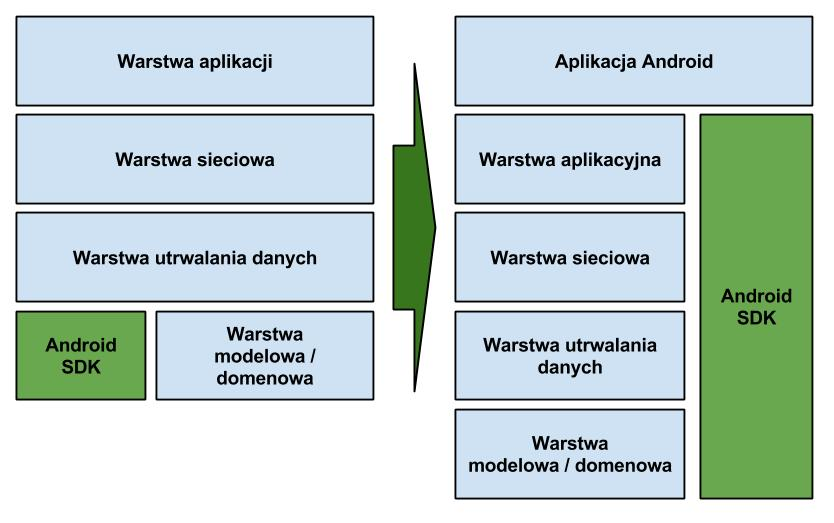
\includegraphics[width=13cm]{imgs/ch4_opis_rozwiazania_1_pl.jpg}
    \caption
{Propozycja modyfikacji struktury aplikacji Android.}
    \label{fig:opis_rozwiazania}
\end{figure} 

Nowy model aplikacji oddziela warstwy \textit{Application}, \textit{Networking}, \textit{Persistance} oraz \textit{Model/Domain} od środowiska Android SDK, a~co za tym idzie nie ma potrzeby umieszczać odwołania do tego środowiska praktycznie w~każdym pliku. Dopiero najwyższą warstwą w~hierarchii jest warstwa \textit{Aplikacja Android}. W~takim podejściu należy użyć Androida jako pewnego rodzaju \textit{pluginu} do tworzonej aplikacji i~uniezależnić warstwę logiczną od reszty warstw. Najpierw napisać aplikację, która będzie oddzielona od Android SDK (na przykład w~czystej Javie), następnie dodać zależności do Android SDK i~skompilować całość w~aplikację androidową. W~ten sposób można być przekonanym, że kod, który stanowi podstawę naszej aplikacji, czyli jej logikę działania, zostanie przetestowany w~oddzieleniu od reszty warstw.

\subsection{Zastosowanie techniki \textit{Test Driven Development} \newline przy tworzeniu oprogramowania}
\label{wybor_tdd}
Jak już zauważono w~rozdziale \ref{test_driven_development} dotyczącym metodologii TDD, wytwarzanie oprogramowania zaczynając od testowania powoduje, że zostanie napisanie tylko tyle aplikacji, ile to jest ujęte w~wymaganiach. A~co za tym idzie jej stopień komplikacji zostanie ograniczony do niezbędnego minimum. Zastosowanie tej techniki w~przypadku aplikacji tworzonych pod Android z~wykorzystaniem uporządkowanej architektury pozwoli na zwiększenie testowalności aplikacji. 

\begin{figure}[!htb]
    \centering
    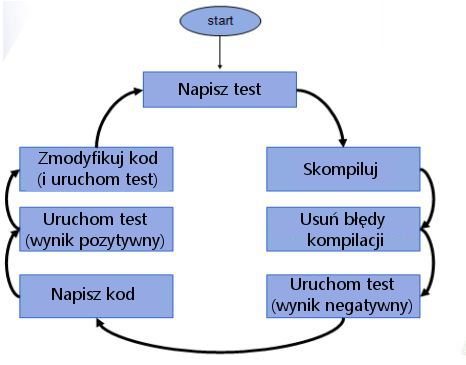
\includegraphics[width=11cm]{imgs/ch4_tdd_pl.jpg}
    \caption
{Schemat pisania programu w~technice \textit{Test Driven Development}.}
    \label{fig:tdd_schema}
\end{figure} 

Korzyści, których można się spodziewać po zastosowaniu tej techniki są następujące:

\begin{itemize}
\item
Wczesne wykrywanie błędów. Odporność na błędy regresyjne. Programista poprawia swoje pomyłki na bieżąco;
\item
Łatwiejszy refaktoring\footnote{Refaktoryzacja (czasem też refaktoring, ang. refactoring) – proces wprowadzania zmian w~projekcie/programie, w~wyniku których zasadniczo nie zmienia się funkcjonalność. Celem refaktoryzacji jest więc nie wytwarzanie nowej funkcjonalności, ale utrzymywanie odpowiedniej, wysokiej jakości organizacji systemu \cite{website:wikipedia}.} kodu;
\item
Dobrze napisane testy stają się dokumentacją kodu;
\item
Lepiej zaprojektowane interfejsy. Technika projektowania testów za pomocą \textit{user stories} zmusza do lepszego przemyślenia rozwiązań i~dokładnego określenia zadań; 
\item
Uproszczona integracja, łatwiejsze łączenie różnych fragmentów kodu poddanych wcześniej testom. Mniej błędów przedostaje się do etapu testów systemowych;
\item
Automatyzacja i~powtarzalność \textit{(contignous integration)}: testy można uruchamiać regularnie o~określonych porach lub na pewnych etapach produkcji; 
\item
Możliwość przetestowania funkcjonalności bez uruchamiania oprogramowania.
\end{itemize}

Wady \textit{Test Driven Development} dotyczą głównie wykorzystania czasu w~projekcie. Wymagany jest:

\begin{itemize}
\item
Dodatkowy czas na stworzenie testów jednostkowych - programista potrzebuje czasem nawet o~40 procent więcej czasu na wykonanie tych samych zadań;
\item
Dodatkowy czas na utrzymanie testów - przy wprowadzaniu zmian w~istniejącej funkcjonalności należy pamiętać, że potrzebny jest również czas na modyfikację istniejących testów jednostkowych.
\end{itemize}

\subsection{Automatyzacja testów jednostkowych}
Testy automatyczne powinny przyczyniać się do poprawy jakości dostarczając szybkiej - dużo szybszej niż w~przypadku testowania manualnego - informacji zwrotnej na temat działania programu. Dodatkowo, szybka informacja zwrotna jest potwierdzeniem, że programista niczego nie uszkodził podczas modyfikowania gotowych funkcji.
Automatyzacja testów nie ma sensu, jeżeli jej koszt jest większy niż korzyści, które przynosi. Z~analizy rysunku \ref{fig:idealna_piramida} z~rozdziału \ref{piramida_testowania} można wnioskować, że największą korzyść przynosi automatyzacja testów jednostkowych. Są relatywnie łatwe do napisania, wykonują się w~ułamkach sekund i~są również łatwe do modyfikacji. Testy jednostkowe są solidną podstawą automatycznych testów regresyjnych.

\subsection{Kod jako dokumentacja programu}
\label{czysty_kod}
Martin Robert Cecil\footnote{Robert Cecil Martin (Uncle Bob) to amerykański inżynier programista oraz autor książek o~programowaniu. Jest również współautorem „Agile manifesto”} - popularny w~środowisku programistycznym \textit{Uncle Bob} - w~\cite{bib:cecil:clean_code}, scharakteryzował dobrze napisany kod następująco: 
\begin{itemize}
\item
Czysty kod można odczytać;
\item
Czysty kod posiada przypisane testy jednostkowe;
\item
Czysty kod posiada znaczące i~rozpoznawalne nazwy zmiennych, klas i~funkcji;
\item
W czystym kodzie poszczególne klasy i~podporządkowane im funkcje robią tylko jedną rzecz;
\item
Czysty kod posiada minimalne zależności, które są wyraźnie zdefiniowane i~zapewniają czyste i~minimalne API;
\item
Czysty kod nie powinien się duplikować;
\item
Czysty kod powinien być "literacki", ponieważ w~zależności od języka nie wszystkie informacje mogą być rozumiane tak samo;
\item
Czysty kod może być łatwo rozbudowany przez inne osoby;
\item
Czysty kod powinien być złożony w~takiej formie, aby był czytelny nie tylko dla maszyny, ale również dla człowieka.
\end{itemize}
Okazuje się jednak, że nie wystarczy raz napisać dobrze kod programu. Jeszcze ciężej jest go utrzymać w~czystej formie podczas rozbudowy aplikacji. Warto więc, zdaniem autora, rozpatrzyć jedno z~nowoczesnych podejść do uporządkowania architektury aplikacji, które może zwiększyć testowalność aplikacji pisanych dla systemu Android.

\section{Praca z~kodem zastanym}
\label{legacy_code}
W rozdziale \ref{pielegnowalnosc_aplikacji} autor nawiązał do problemu pracy z~kodem zastanym, tak zwanym \textit{Legacy Code}.
Co więc zrobić, aby zaimplementować testy do już napisanego kodu? Godfrey Nolan\footnote{Godfrey Nolan - założyciel i~prezes RIIS LLC, firmy zajmującej się rozwojem oprogramowania dla platform przenośnych. Autor książek o~Androidzie: "Agile Android", "Booletproof android", "Android Best Practices" i~"Decompiling Android"} w~swojej książce "Agile Android" \cite{bib:agile:android} proponuje następujące rozwiązanie:

\begin{itemize}
\item 
Wprowadzić metodę ciągłej integracji w~procesie budowania kodu -  (\textit{Continuous Integration (CI)});

Jest to należąca do metodologii zwinnych praktyka polegająca na regularniej integracji zmian w~kodzie do bieżącego repozytorium. Warunkiem koniecznym umieszczenia kodu w~repozytorium jest upewnienie się, że dany kod działa;

\item
Bezwzględnie pisać testy jednostkowe do nowych części oprogramowania zgodnie z~TDD, \textit{mockując} jeśli to możliwe wykorzystywane obiekty z~zastanego kodu;

\item
Skorzystać z~serwera CI (dobrym przykładem jest tutaj \textit{Jenkins}\footnote{http://jenkins-ci.org/}), który będzie wykonywał testy jednostkowe, do których istnieje przekonanie, że ich implementacja nie powinna się zmieniać. Należy pamiętać, że~testy automatyczne muszą również podlegać przeglądom;

\item
Uświadomić zespół programistów na czym polegają testy jednostkowe i~przekonać ich do stosowania TDD;

\item
Dodać metryki mierzenia kodu do CI. Ustawić poziom minimalny na 10-15\%;

\item
Użyć frameworka do podstawowych testów GUI już istniejącej aplikacji. Stworzyć testy opierając się na przypadkach użycia (ang. \textit{use cases)};

\item
Wyizolować zastany kod, tak aby nikt z~programistów nie miał do niego dostępu, jeżeli naprawdę nie jest to niezbędne;

\item
Usunąć niewykorzystywane i~nieużyteczne części kodu;

\item
Przepisać i~przetestować wyizolowany kod, aby zwiększyć metryki pokrycia do około 60-70\%. 
\end{itemize}

Najważniejsze więc jest wyizolować stary kod, przetestować aplikację za pomocą frameworka do testów GUI, usunąć ewentualne błędy nie pozwalające na poprawną pracę programu i~nie modyfikować wyizolowanego kodu podczas pisania nowych funkcjonalności. Nowe funkcje należy dodawać stosując już taktykę \textit{Test Driven Development}. Dopiero na końcu, jeżeli tworzone środowisko jest już stabilne, należy rozpocząć przebudowę starych części aplikacji, tak aby metryki pokrycia kodu rosły wraz z~upływem czasu. Przy wykonywaniu \textit{refaktoringu} Godfrey Nolan proponuje użyć narzędzia \textit{SonarQube\footnote{SonarQube - platforma do prowadzenia ciągłej inspekcji jakości kodu źródłowego, dostarczana na licencji \textit{open source}}}.

\section{Różne podejścia do uporządkowania architektury}
\subsection{Architektura cebulowa - \textit{The Onion Architecture}}
Jeffrey Pallermo w~połowie 2008 roku opublikował na swoim blogu serię artykułów  \cite{website:architect:onion}, w~których zaproponował inne od klasycznego podejście do warstw w~aplikacji. Zauważył, że uzależnienie warstwy biznesowej od warstwy danych niekorzystnie wpływa na stabilność warstwy biznesowej, która z~założenia powinna być niezależna od wprowadzania nowych technologii do warstwy bazodanowej. Stare podejście tego nie zapewniało. W~większości przypadków warstwa biznesowa musiała być modyfikowana, a~przynajmniej rekompilowana podczas modyfikacji warstwy dostępu do danych.

W zaproponowanym przez Palermo modelu, im warstwy położone są w~architekturze głębiej, tym mniej podatne są na zmiany. Zależności mogą być zwrócone tylko w~jedną stronę - do wnętrza "cebuli". w~ten sposób w~centrum znajdzie się model domeny, a~na zewnątrz - warstwa bazodanowa. Jest to podejście nazywane \textit{odwróceniem zależności\footnote{Dependency Inversion Principle (DIP) - zasada mówiąca, że moduły wysokopoziomowe nie powinny zależeć od modułów niskopoziomowych. Obie grupy powinny zależeć od abstrakcji. Abstrakcje natomiast nie powinny zależeć od szczegółowych rozwiązań, tylko odwrotnie.}} i~wymaga od programistów zastosowania odpowiednich technik projektowych, między innymi \textit{wstrzykiwania zależności\footnote{Dependency Injection (DI) – wzorzec projektowy i~wzorzec architektury oprogramowania polegający na usuwaniu bezpośrednich zależności pomiędzy komponentami na rzecz architektury typu plug-in \cite{website:wikipedia}.}}.

Warstwy wewnętrzne definiują interfejsy, za pomocą których mogą komunikować się z~warstwami zewnętrznymi. Dzięki temu programiści nie muszą implementować na przykład dostępu z~warstwy biznesowej do bazy danych w~warstwie danych, zaimplementują tylko odpowiedni interfejs.

\begin{figure}[!htb]
    \centering
    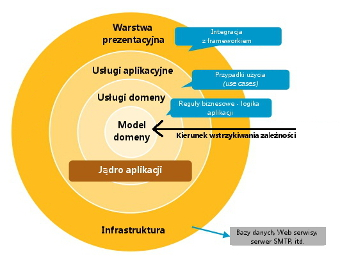
\includegraphics[width=11cm]{imgs/ch4_onion_architecture_pl.jpg}
    \caption
{\textit{Onion architecture} według Jeffrey'a Palermo  \cite{website:architect:onion}.}
    \label{fig:onion_architecture}
\end{figure} 

Kluczowe założenia architektury cebulowej (rysunek \ref{fig:onion_architecture}):
\begin{itemize}
\item 
Aplikacja zbudowana jest według niezależnego modelu obiektowego;
\item
Warstwy wewnętrzne definiują interfejsy. Warstwy zewnętrzne te interfejsy implementują;
\item
Kierunek \textit{sprzężenia} jest od warstwy zewnętrznej do wewnętrznej;
\item
Cały kod rdzenia aplikacji (\textit{Object Model, Object services, Application Services}) może zostać skompilowany i~wykonany bez kontaktu z~infrastrukturą i~interfejsem użytkownika.
\end{itemize}


\subsection{Architektura portów i~adapterów - \textit{Ports and Adapters \newline Architecture}}
Opracowana w~2005 roku przez Alistaira Cockburna\footnote{Alistair Cockburn - jeden z~inicjatorów ruchu Agile. Jest współautorem wydanego w~2001 roku manifestu Agile. w~roku 2005 pomagał współtworzyć deklarację 'PM Declaration of Interdependence'. Propagator przypadków użycia jako dokumentacji procesów biznesowych oraz wymagań co do zachowania oprogramowania \cite{website:wikipedia}.} architektura niegdyś znana była pod nazwą architektury heksagonalnej \cite{website:architect:hexagonal}. Nazwa \textit{"heksagonalna"} przyjęła się, ponieważ kiedyś znane były tylko trzy porty wejściowe i~trzy porty wyjściowe, stąd wszystkie schematy rysowane były jako foremny sześciokąt. Wraz ze wzrostem liczby portów wejściowych i~wyjściowych zmieniono nazwę na \textit{Ports \& Adapters}, nie zmieniono natomiast zasady przedstawiania architektury na schematach, co przedstawia rysunek \ref{fig:hexagonal_architecture}.

\begin{figure}[!htb]
    \centering
    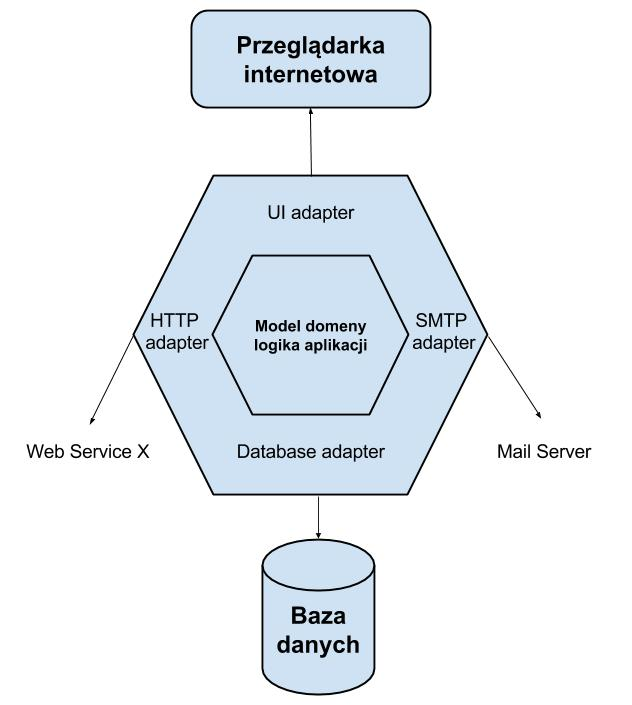
\includegraphics[width=10cm]{imgs/ch4_hexagonal_architecture_3.jpg}
    \caption
{Architektura heksagonalna według Alistaira Cockburna.}
    \label{fig:hexagonal_architecture}
\end{figure} 

Idea jest bardzo podobna do architektury cebulowej: w~centrum znajduje się jądro aplikacji, czyli model domeny i~logika biznesowa, odpowiedzialna za kluczowe działania programu. Jądro otoczone jest przez warstwę portów, zawierającą porty zarówno wejściowe, jak i~wyjściowe. Zewnętrzną warstwą jest warstwa adapterów.

\paragraph{Jądro - \textit{Kernel}}
Jądro oferuje model domeny i~logikę biznesową: ogólne możliwości aplikacji, operacje, logikę operacji oraz mechanizmy wspierania decyzji, co już w~wymienionej kolejności stanowi architekturę warstwową. Warstwa również może być podzielona na kilka poziomów logiki. 

\paragraph{Porty - \textit{Ports}}
Porty są to interfejsy usług: API, odczyt danych (wejściowe), oraz interfejsy repozytoriów czy DAO\footnote{Data Access Object – komponent dostarczający jednolity interfejs do komunikacji między aplikacją a~źródłem danych.}, sterowniki do różnego rodzaju maszyn, urządzeń, odbiorników GPS czy radia (wyjściowe). Za pomocą portów wyjściowych warstwa jądra jest w~stanie emitować zdarzenia. Zdarzenia są techniką odwracania kontroli, czyli działają z~zachowaniem wspomnianej już zasady, że warstwa wewnętrzna nie posiada kontroli nad warstwą zewnętrzną. 

\paragraph{Adaptery - \textit{Adapters}}
Szczególnym przykładem adaptera jest aplikacja webowa, która z~jednej strony komunikuje się z~serwerem baz danych, a~z drugiej z~cienkim klientem\footnote{Cienki klient (ang. thin client) – komputer bądź specjalizowane urządzenie (terminal komputerowy) wraz z~odpowiednim oprogramowaniem typu klient, umożliwiające obsługę aplikacji stworzonej w~architekturze klient-serwer. Cechą szczególną cienkiego klienta jest niezależność od obsługiwanej aplikacji serwerowej (jej zmiana nie pociąga za sobą konieczności wymiany oprogramowania klienta). Dodatkowym atutem jest niewielkie zapotrzebowanie na moc przetwarzania \cite{website:wikipedia}.}, jakim jest na~przykład przeglądarka internetowa po stronie użytkownika. Może odbierać również zdarzenia od innych modułów systemowych, jeżeli architektura systemowa jest modułowa (Listener/Receptor zdarzeń). Głównym zadaniem adapterów jest delegowanie zdarzeń do portów na warstwie położonej wewnątrz i~powinno się w~miarę możliwości unikać przypisywania adapterom większej ilości zadań.

Z punktu widzenia systemu napisanego w~architekturze cebulowej, testowalność oprogramowania wygląda następująco: testy jednostkowe eksplorują warstwę \textit{Kernel} zawierającą model domeny i~logikę biznesową, testy integracyjne sprawdzają porty, a~testy systemowe badają kilka warstw \textit{Kernel} na raz.

\subsection{Architektura uporządkowana - \textit{The Clean Architecture}}
\label{clean_architecture_opis}
Cytowany już w~rozdziale \ref{czysty_kod} Uncle Bob opublikował w~2012 roku na swoim blogu propozycję usystematyzowania architektury systemowej  \cite{website:cecil:blog}, która zainteresowała również autora tej pracy. Schemat architektury uporządkowanej przedstawiony jest na rysunku \ref{fig:clean_architecture}.
\newpage

\begin{figure}[!htb]
    \centering
    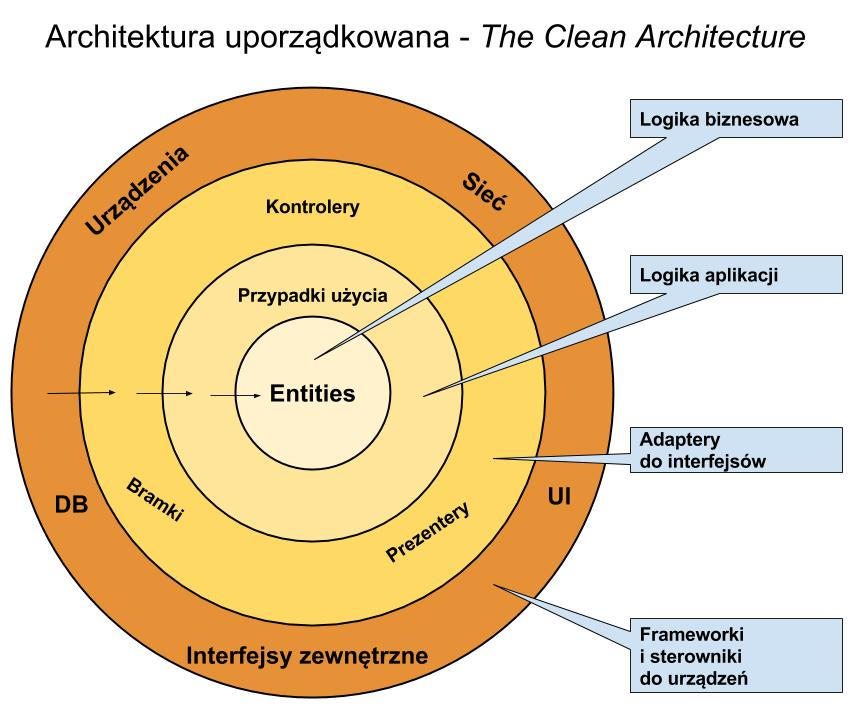
\includegraphics[width=12cm]{imgs/ch4_clean_architecture_pl.jpg}
    \caption
{Clean architecture of Android według Uncle Bob  \cite{website:cecil:blog}.}
    \label{fig:clean_architecture}
\end{figure} 

Idea tego rozwiązania jest następująca:

\begin{itemize}

\item
Najważniejszym elementem jest środek, czyli warstwa \textit{Entities}. w~warstwie tej znajdują się kluczowe dla tworzonej aplikacji reguły biznesowe gwarantujące poprawność działania programu - logika działania aplikacji;
\item
Drugą warstwą jest \textit{Use Cases} - \textit{przypadki użycia}, ale bardziej adekwatną jest nazwa \textit{intencje biznesowe}. Jest to zbiór wszystkich zachowań, jakich oczekuje się od tworzonego systemu. W~przypadku aplikacji bankowej, może być to na przykład funkcja wykonywania przelewu, jako jeden przypadek użycia, a~innym takim przypadkiem byłoby sprawdzenie stanu konta;
\item
Wyższa, otaczająca warstwa dotyczy wszystkich kontrolerów i~prezenterów; 
\item
Dopiero na ostatniej, najbardziej zewnętrznej warstwie pojawia się powiązanie z~Android SDK. Wykorzystywane jest, aby dostać się do baz danych, skorzystać z~interfejsów użytkownika dla danego urządzenia oraz uzyskać dostęp do zewnętrznych interfejsów lub urządzeń.
\end{itemize}

Warstwy na schemacie połączone są strzałkami, które informują o~kierunku przepływu informacji. Ze schematu wynika, że warstwa \textit{Entities} nie posiada informacji o~istnieniu \textit{Use Cases}, \textit{Use Cases} nie posiadają informacji o~kontrolerach i~prezenterach, a~te z~kolei nie wiedzą o~istnieniu interfejsu użytkownika. Patrząc w~drugą stronę, każda warstwa wyższa posiada wszystkie informacje o~warstwie niższej, czyli \textit{UI} wie wszystko o~prezenterach, te wiedzą wszystko o~\textit{Use Cases}, a~przypadki użycia mogą korzystać z~wiedzy o~całej warstwie logicznej.

Podsumowując, jeżeli programista używa powiązania z~Android SDK, to tylko z~poziomu najwyższej warstwy. Nie należy tego robić w~stosunku do warstwy niższej, bo wtedy cała koncepcja może ulec dezintegracji.

W ten sposób teoretycznie można stworzyć architekturę, która:
\begin{itemize}
\item
jest niezależna od frameworka (tutaj Android SDK) i~zachowana zostaje zasada zależności;
\item
jest niezależna od \textit{UI}, bazy danych lub innych urządzeń zewnętrznych;
\item
jest testowalna, w~oderwaniu od warstwy zawierającej interfejsy wymienione powyżej.
\end{itemize}

Jeżeli struktura tworzonej aplikacji zostanie ułożona w~powyższy sposób – testowanie (przynajmniej jednostkowe) nie powinno być bardziej skomplikowane niż w~przypadku kodu napisanego w~czystej Javie czy C++.
